\begin{figure}[t]
  \centering
  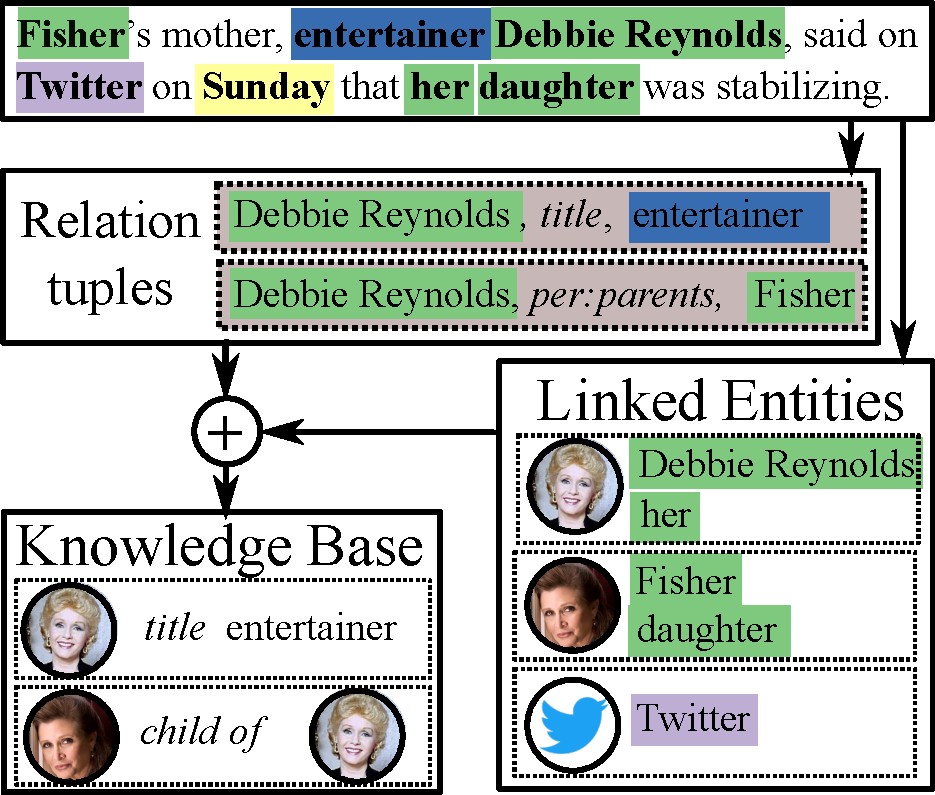
\includegraphics[width=0.9\columnwidth]{figures/entities-example.pdf}
  \caption{\label{fig:example} An example describing entities and relations in knowledge base population. \ac{Change tuple to instance. Potentially make figure less ugly.}}
\end{figure}

\section{Introduction}
\label{sec:intro}

% (1 page w/ figure)
% Goal: remind the reader what information extraction is, what its relation to knowledge base population is and why it is important. Hook question.
Harnessing the wealth of information present in unstructured text online has been a long standing goal for the natural language processing community.
In particular, knowledge base population seeks to automatically construct a knowledge base consisting of relations between entities from a document corpus (\reffig{example}).
Knowledge bases have found many applications including question answering \citep{berant2013freebase, fader2014open,reddy2014large}, automated reasoning \citep{kalyanpur2012structured} and dialogue~\citep{lee2015conversational,han2015exploiting}.

% Evaluation @ scale poses problem. -- pooling methodology
Evaluating these systems remains a challenge as it is not economically feasible to exhaustively annotate every possible candidate relation from a sufficiently large corpus.
As a result, a pooling-based methodology is used in practice to construct datasets, similar to them methodology used in information retrieval \citep{sparck1975report, harman1993trec}.
For instance, at the annual NIST TAC KBP evaluation, all relations predicted by participating systems are pooled together, annotated and released as a dataset for researchers to develop and evaluate their systems on.
However, during development, if a new system predicts a previously unseen relation it is considered to be wrong even if it is correct.
The discrepancy between a system's true score and the score on the pooled dataset is called pooling bias and is typically assumed to be insignificant in practice \pl{any citations or quotes backing this assumption?}.

% Key finding: pooling bias
The key finding of this paper contradicts this assumption and shows that the pooling bias is actually significant, and it penalizes newly developed systems by 2\% \fone{} on average (\refsec{analysis}).
Novel improvements, which typically increase scores by less than 1\% \fone{} on existing datasets, are therefore likely to be clouded by pooling bias during development.
Worse, the bias is larger for a system which predicts qualitatively different relations systematically missing from the pool.
% anti-solution
Of course, systems participating in the TAC KBP evaluation do not suffer from pooling bias, but this requires researchers to wait a year to get credible feedback on new ideas.
% TODO: I would like to add something about how ML methods are hosed, but perhaps for later?
%This bias is particularly damaging for any machine learning method as it is actively discouraged from predicting unseen relations and learning novel patterns.
The net effect is that researchers are discouraged from developing innovative approaches, thereby slowing progress on the task.
%These observations may explain why rule-based systems still play such a significant role in the top submissions at TAC KBP, and why, even after 8 years, top automated systems achieve scores of only about 35\% \fone{} while human annotators score above 60\% \fone{} on the same task.

% Solution: on-demand evaluation.
To address this, in \refsec{method}, we propose a new evaluation methodology, \emph{on-demand evaluation},
which avoids pooling bias by querying crowdworkers,
but to minimize cost, we do it selectively, leveraging previous systems' predictions when possible.
%When a researcher submits a new system's predictions to our evaluation platform,
%we carefully sample a subset of its predictions and have crowdworkers judge them.
%just enough of its predictions to guarantee an accurate estimate of scores and have crowdworkers judge them.
We then compute the new system's score based on the predictions of past systems using importance weighting \pl{optional: say half a sentence more about this}.
As more systems are evaluated, the marginal cost of evaluating a new system decreases.
% Experimental results.
We simulate our method on evaluation data released through the TAC KBP 2015 Slot Validation track and show that we are able to obtain unbiased estimates of a new systems score's while reducing variance.

Our second contribution is an implementation of our framework as a publicly available evaluation service\footnote{\url{https://anonymo.us}} where researchers can have their own KBP systems evaluated.
We pilot this service by evaluating three distinct systems on the 2016 TAC KBP corpus for about \$300 a system (a fraction of the cost of official evaluation).
We believe the instance of this service will speed the pace of progress in developing KBP systems.
\ac{This number is a bit tangential to our contribution: our costs are amortized over time and we aren't able to show that here}. \ac{Also unsure about what else to say about the evaluation.}
\pl{if this is meant to be a contribution, should say more about what the
conceptual gap is between coming up with the estimator and creating this
service...or say something about the intended use case of this service (for development)?}
%availability of will help accelerate the development of better knowledge base population systems.

%and find that we are able to estimate precision and recall to within about 2\% \fone{} (\fake{a third the variance as official scores}) and within a budget of \$3000 (a fraction of the cost of the official evaluation). 

%%% vvv OLD as of 4/8/17

%% II. 
%% 1. KBP as case study -- what is KBP?
%% TODO: is this too much detail?
%%Before elaborating, let's look at how knowledge base population (KBP) is evaluated.
%\pl{found this transition jarring - we already talked about evaluation, only now defining KBP;
%define KBP first?}
%\pl{Can we use 'relation instance' from the get go?
%The problem is so clear and simple when described in terms of intersections of sets of relation instances
%in a way that it's not when talking about KBs, corpuses, entities, relations, etc.
%}
%In KBP, a system is given a large document corpus and must output a knowledge base (KB) consisting of entities and relations mentioned in the corpus, e.g.\ ``Carrie Fisher's mother is Debbie Reynolds'' or ``Carrie Fisher was born in Los Angeles'' (\figureref{task}). % according to a specified schema.
%These predicted KBs are evaluated on how accurately they predict relations for an entity (precision) \pl{define this more precisely} and how many of these relations they are able to correctly predict (recall), using an evaluation set and the closed-world assumption. %TODO: need a name for this set.
%
%% III.
%% 2. How is KBP evaluated? -- pooled eval, closed world assumption, output evaluated for a window.
%The primary source of evaluation data for KBP comes from the annual TAC KBP competition organized by NIST.\@ %~\citep{}. % TODO: add links to workshop overview papers
%Each year, teams submit their predicted KBs for a given document corpus.
%Selected output \pl{use something more specific than 'output' - 'relations'} is annotated by the organizers and released to help researchers develop better systems.
%% TODO: while not biased for entrants in the competition, development sucks.
%% - we measure pooling bias
%Unfortunately, under the closed world assumption, new predictions that development systems make are not part of this evaluation data and are assumed to be wrong.\footnote{%
%It is also possible to simply ignore new predictions during evaluation, but this has the reverse effect of gratuitously inflating scores by about \fake{3\%} on average according to our analysis.}
%% - why it matters: effect on novel predictions -- hurts new ideas!
%We estimate that this bias causes development \fone{} scores to be on average 2\% points lower than they should be, while significant improvements usually increase scores by less than 1\% \fone{}.
%Worse yet, the more novel a system is \pl{claim warrants elaboration - say system predicts qualitatively different things that were systematically missed before}, the stronger the bias against it will be, potentially even causing scores to drop.
%% - while rule-based systems are robust because of human guidance -- empirically driven -- directs any output to what is already
%While designers of rule-based systems can still look to their intuition for guidance, those who rely on empirical tuning and machine learning are, at best, left in the dark, and more likely to be directed towards only predicting what others have predicted and no more.
%
%% - might explain great KBP stagnation -- bad scores and pattern based systems still leading -- cite system reports.
%Of course, relations predicted by systems participating in the competition are fairly evaluated and do not suffer from any bias, but this requires researchers to wait a year to get credible feedback on new ideas.
%%
%These observations may explain why rule-based systems still play such a significant role in the top submissions at competition, and why, even after 5 years of running the competition, top automated systems achieve scores of only about 35\%\fone{} while human annotators score above 60\%\fone{} on the same task.
%
%%What, then, can be done to address this problem?
%To address this bias, we propose a new on-demand evaluation based on crowdsourcing.
%%We propose a new evaluation framework in which predicted KBs submitted by researchers are suitably sampled and evaluated through crowd-sourcing.
%Upon receiving a new system's predictions, crowdworkers evaluate a sample of these predictions to provide an estimate of precision and recall.
%%We estimate recall of the system against a carefully-chosen subset of documents in the corpus,
%%  which has been exhaustively annotated in advance.
%The key challenges we address are cost, ensuring coverage of entities and relations and ensuring unbiased estimates.
%For the first, the framework leverages the fact that it is much cheaper to \textit{verify} relations than it is to find them within a large corpus.
%For the second, we employ a structured sampling scheme to reduce the variance of entity-level and recall-level precision and recall.
%Finally, we exhaustively annotate a few documents to de-bias our recall estimates in a cost-effective manner.
%
%%To address this bias, we propose a new on-demand evaluation based on crowdsourcing.
%%Upon receiving a new system's predictions,
%%crowdworkers evaluate a sample of these predictions to provide an unbiased estimate of precision.
%%We estimate recall of the system against a carefully-chosen subset of documents in the corpus,
%%which has been exhaustively annotated in advance.
%%We also perform careful sampling and reweighting to further reduce the variance of our estimates.
%
%
%% I think pooling bias isn't necessarily what people will think of first, so moving this to related work / discussion.
%% This ``pooling'' bias has also been identified in the information retrieval community\needcite, which bears many similarities to the knowledge base population task, e.g.\ both tasks seek to find ``relevant'' information from a large document corpus that is infeasible to exhaustively annotate.
%% However, assessing the quality of system outputs is relatively objective in the context of knowledge base population.
%% This enables us to employ non-expert crowdworkers to accurately judge novel output submitted by teams during development.
%
%We simulate this framework on a mock evaluation of three distinct systems on the 2016 TAC KBP corpus and find that we are able to estimate precision and recall within \fake{2\%} \fone{} (half as much as the official scores) and within a budget of \fake{\$2000} (a fraction of the cost of the official evaluation).\footnote{%
%  The implementation of the online evaluation platform will be made available for submissions at \url{http://anonymo.us}.
%}
%We hope that the immediate, unbiased evaluation
%will help accelerate the development of better information extraction systems.
%
%%\begin{figure}[t]
%%  \includesvg[width=\columnwidth]{figures/entites-example}
%%  \caption{\label{fig:example}
%%  What do KBP outputs look like?
%%  }
%%\end{figure}
%
%%A number of confounding factors affect performance, including the performance of other systems, making comparisons difficult.
%% Analysis: biased!
%%We begin with a statistical analysis of the KBP evaluation in \sectionref{analysis},
%%and find that the pooling evaluation that teams use during development
%%produces scores that are on average 2\% points lower than they should be.
%%The source of this \emph{pooling bias}, also studied in the information retrieval community \needcite,
%%is the closed-world nature of the evaluation:
%%any predictions that fall outside the previous systems' predictions,
%%even correct ones, are incorrectly labeled as negative.
%%This evaluation is thus biased against novel system improvements!
%
%% PL: simplified
%%The source of this bias arises because
%%the evaluation data only contains assessments for a subset of every candidate fact in the corpus
%%and there is no good way to score a predicted fact that is not part of this subset.
%%In particular, the evaluation data consists only of the candidate facts
%%``pooled'' together from systems that participated during the original
%%competition and were subsequently assessed by human annotators.
%
%% Describe pooling bias, connect to IR
%%This bias has been studied in the information retrieval community\needcite,
%%which bears many similarities to the knowledge base population task,
%%e.g.\ both tasks
%%which also seeks to find ``relevant'' information from a large document corpus that is infeasible to exhaustively annotate.
%
%% Our solution
%% To address this bias, we propose a new on-demand evaluation based on crowdsourcing.
%% Upon receiving a new system's predictions,
%% crowdworkers evaluate a sample of these predictions to provide an unbiased estimate of precision.
%% We estimate recall of the system against a carefully-chosen subset of documents in the corpus,
%% which has been exhaustively annotated in advance.
%% We also perform careful sampling and reweighting to further reduce the variance of our estimates.
%%However, assessing the quality of system outputs is relatively objective in the context of knowledge base population.
%%This enables us to employ non-expert crowdworkers to accurately judge novel output submitted by teams during development.
%% PL: I'm not sure the 'objective, therefore crowdsourcing' is convincing - 'relevance' also lends itself to crowdsourcing, which is what is done in IR too;
%
%% Results
%%We simulate this evaluation protocol on the 2015 \plg{abstract says 2016} KBP challenge.
%%We find that we are able to confidently evaluate submissions within a budget of \fake{\$100/system} with a fixed cost of \fake{\$1000/corpus} \plg{per document?}.\footnote{The implementation of the online evaluation platform will be made available for submissions at \url{http://anonymo.us}.}
%%The practical on-demand evaluation also addresses
%%the slow feedback loop that researchers face in testing their developments: they
%%must wait a year for the next TAC KBP challenge followed by several months to
%%receive their test scores.  We hope that the immediate, unbiased evaluation
%%will help accelerate the development of better information extraction systems.
%%
%%\plg{might want to incorporate some of this material into the preceding paragraphs}
%%(scrap material)
%%We propose a new online evaluation protocol that automates the process of query selection to provide more precise estimates of instance-level and entity-level evaluation metrics than the current methodology.
%%The evaluation protocol uses a careful combination of annotation of pooled output, exhaustive annotation on a subset of documents and correlations between unassessed outputs to produce unbiased estimates of precision and recall.
%%
%%\plg{would probably drop this or fold it in - seems to minor to standalone}
%%Of independent interest is a statistical analysis of submissions to past KBP challenges that allows us to make comparisons across years.
%%%>>>>>>> e07c734e841131ffe898f7af72ea71f63bbb33e1
%%
%%\plg{we had talked about arguing why static datasets don't quite help;
%%do we have anything to say there?}
%
%%The platform is easy to use and will have a fresh stream of documents.
%
%%For these reasons, we propose and implement a new evaluation methodology: an online evaluation platform that teams can submit to as they develop their systems (\sectionref{design}).
%%We use a combination of exhaustive, selective and estimative annotations to balance cost, accuracy and guaranteed unbiased estimates of precision, recall and $\fone$ scores at the mention and entity level.
%% \plg{I don't see the 'online evaluation platform' as the immediate solution;
%% what I'd expect is a more technical solution - how to do the crowdsourcing to deal
%% with bias and reweighting to deal with variance;
%% making it online seems to help with more community aspects,
%% which can be argued as valuable, but that seems like a separate point}
%
%%\cite{chaganty2016perspectives}
%
%%Next, we measure the effect of the pooling methodology \pl{need to explain pooling in enough detail for people to appreciate the problem} and find that it is significantly biased against unpooled systems: when evaluating improvements to your KBP system, your scores on the evaluation data could be 4--7\% lower than they would be if you had submitted said system; if you are developing a new KBP system, the bias can be as much as 20\%.
%%This is serious methodological problem that provides a barrier of entry for new teams and makes incremental improvements to systems a coin toss-- real improvements in results will easily pass unnoticed. 
%
%
%% We find that there is a large amount of variance in the scores due to varying difficulties of the query entities which leads to wide confidence intervals on the reported results.
%% We show that this variance can be reduced by standardizing scores across queries, a new metric that is able to discriminate between systems \todo{50\%} more effectively. 
%% \pl{the variance doesn't seem to be the thing causing the plateau;
%% certainly it doesn't explain the difference between 30\% and 80\%;
%% seems the bias is more pressing and should be talked about first
%% }
%
%
%% TODO: We haven't tried doing a cross-evaluation yet -- this would basically mean we take a reference system and try and compare performance across years relative to this system.
%% We use a method for score standarization (\refsec{analysis}) to compare scores across years and find that \todo{there is no statistically significant improvement in the last several years}.
%
